\section{视网膜的信息处理}
\subsection{外网状层的信息传递}
\begin{frame}
    \frametitle{外网状层的信息传递\label{frame1}}

    光感受器在在\textbf{黑暗环境下去极化},并释放神经递质(据认为是谷氨酸)。

    在外网状层,每个光感受器都和两种视神经元:双极细胞和水平细胞形成突触。
    其中,双极细胞构成自感受器到神经节细胞的直接通路。
    水平细胞负责外网状层信息的侧向传递,以影响其临近的双极细胞的活动性。

    基于对神经递质的反应,双极细胞分为两类:
    \begin{itemize}
        \item \textbf{撤光双极细胞}(OFF bipolar cell)谷氨酸门控阳离子通道通过$Na^+$的内流,介导经典的去极化的兴奋性突触。
        \item \textbf{给光双极细胞}(ON bipolar cell)对谷氨酸的响应为超极化。
    \end{itemize}
    OFF和ON的定义在于这些细胞是否对撤光(更多谷氨酸)或给光(少谷氨酸)产生去极化影响。
    双极细胞的\textbf{感受野}(receptive field)是视网膜上给光刺激能改变细胞膜电位的区域。
    
\end{frame}

\begin{frame}
    \frametitle{双极细胞的感受野}

    \begin{columns}
        \column{.5\textwidth}{
            双极细胞的感受野由两部分组成:
            \begin{itemize}
                \item 一个提供直接光感受器输入的圆形视网膜区域,称为感受野中心。
                \item 以及一个通过水平细胞提供输入的视网膜的环形区域,称为感受野周边。
            \end{itemize}
            感受野越靠近中心越小,越靠近周边越大。
        }\column{.5\textwidth}{
            \begin{figure}
                \centering
                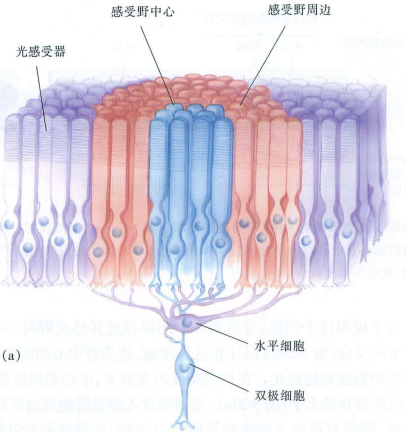
\includegraphics[width=.8\textwidth]{img/pic6-1.png}
                \caption{细胞连接示意图\label{pic6-1}}
            \end{figure}
        }
    \end{columns}

\end{frame}

\begin{frame}
    \frametitle{信号传递通路}

    \begin{columns}
        \column{0.5\textwidth}{
            在感受野中心的光通过直接通路给光中心型的双极细胞\textbf{去极化};
            在感受野周边的光通过简介通路给光中心型双极细胞\textbf{超极化}。

            由于水平细胞的介入,光对周边光感受器的作用总是与其对中心光感受器的作用相反。
            我们称这些细胞具有颉颃的\textbf{中心-周边感受野}
        }\column{.5\textwidth}{
            \begin{figure}
                \centering
                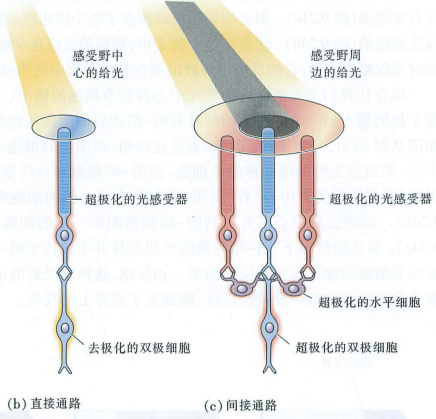
\includegraphics[width=\textwidth]{img/pic6-2.png}
                \caption{直接通路与间接通路\label{pic6-2}}
            \end{figure}
        }
    \end{columns}
    \scriptsize{Tip:图\ref{pic6-2}仅仅是幻灯片\ref{frame1}提到双极细胞的一种,
    另一种的去/超极化过程与其相反。}

\end{frame}


